\documentclass[a4paper]{article}
\usepackage[utf8]{inputenc}
\usepackage{textcomp}
\usepackage{geometry}
\geometry{ left=2cm, right=2cm, top=2cm, bottom=4cm, bindingoffset=5mm}
\usepackage{graphicx}
\usepackage{xcolor}
\usepackage{hyperref}
\date{}
\author{}
\usepackage{fancyhdr}
\pagestyle{fancy}
\fancyhf{}
\fancyhead[R]{2973140 - Felix Bühler \\ 2892258 - Gerhard Breul \\  3141241 - Jamie Ullerich}
\fancyhead[L]{Information Visualisation and Visual Analytics \\ WS 2019/20 }
\renewcommand{\headrulewidth}{0.5pt}
\usepackage{tikz}
\usetikzlibrary{calc}
\usepackage{amsmath}
\usepackage{cleveref}
\usepackage{subcaption}

\usepackage{changepage,lipsum,titlesec}
\titleformat{\section}[block]{\bfseries}{\thesection.}{1em}{}
\titleformat{\subsection}[block]{}{\thesubsection}{1em}{}
\titleformat{\subsubsection}[block]{}{\thesubsubsection}{1em}{}
\titlespacing*{\subsection} {2em}{3.25ex plus 1ex minus .2ex}{1.5ex plus .2ex}
\titlespacing*{\subsubsection} {3em}{3.25ex plus 1ex minus .2ex}{1.5ex plus .2ex}


\title{\textbf{Assignment 8}}

\begin{document}
\maketitle 
\thispagestyle{fancy}

\section*{Task 1 - The happiness index by country}
\subsection*{(a) Visualizing the data}
%In either case, reflect and report in 3-10 sentences on the message of your poster/dashboard: if it is a storytelling assignment, what is the point of view you are conveying? if it is a data exploration assignment, what are potential conclusions an external viewer of your visualization might reach upon inspecting/reading your poster?
Our poster consists of three parts: there is a map at the top which shows the happiness score for each country on a map. 
This is supposed to give a quick overview on how the happiness is distributed across the world. 
Of course, this does not show any detail on the exact scores, therefore we created the more detailed visualisations at the bottom. 
Left, there is a bar chart which shows the ten happiest and least happy country. 
The ranking can be easily seen, as well as the difference between each country. 
Besides that, it shows the composition, which is also interesting, because it is possible to compare if one of the influencing factors is less or more present in happy or rather sad countries. 
So, these two visualisations cover the happiness score and how it is composed in detail. 
TODO visualisation 3. 

% Briefly report on weaknesses and strengths of your visualization, as well as potential improvements.
TODO

\fbox{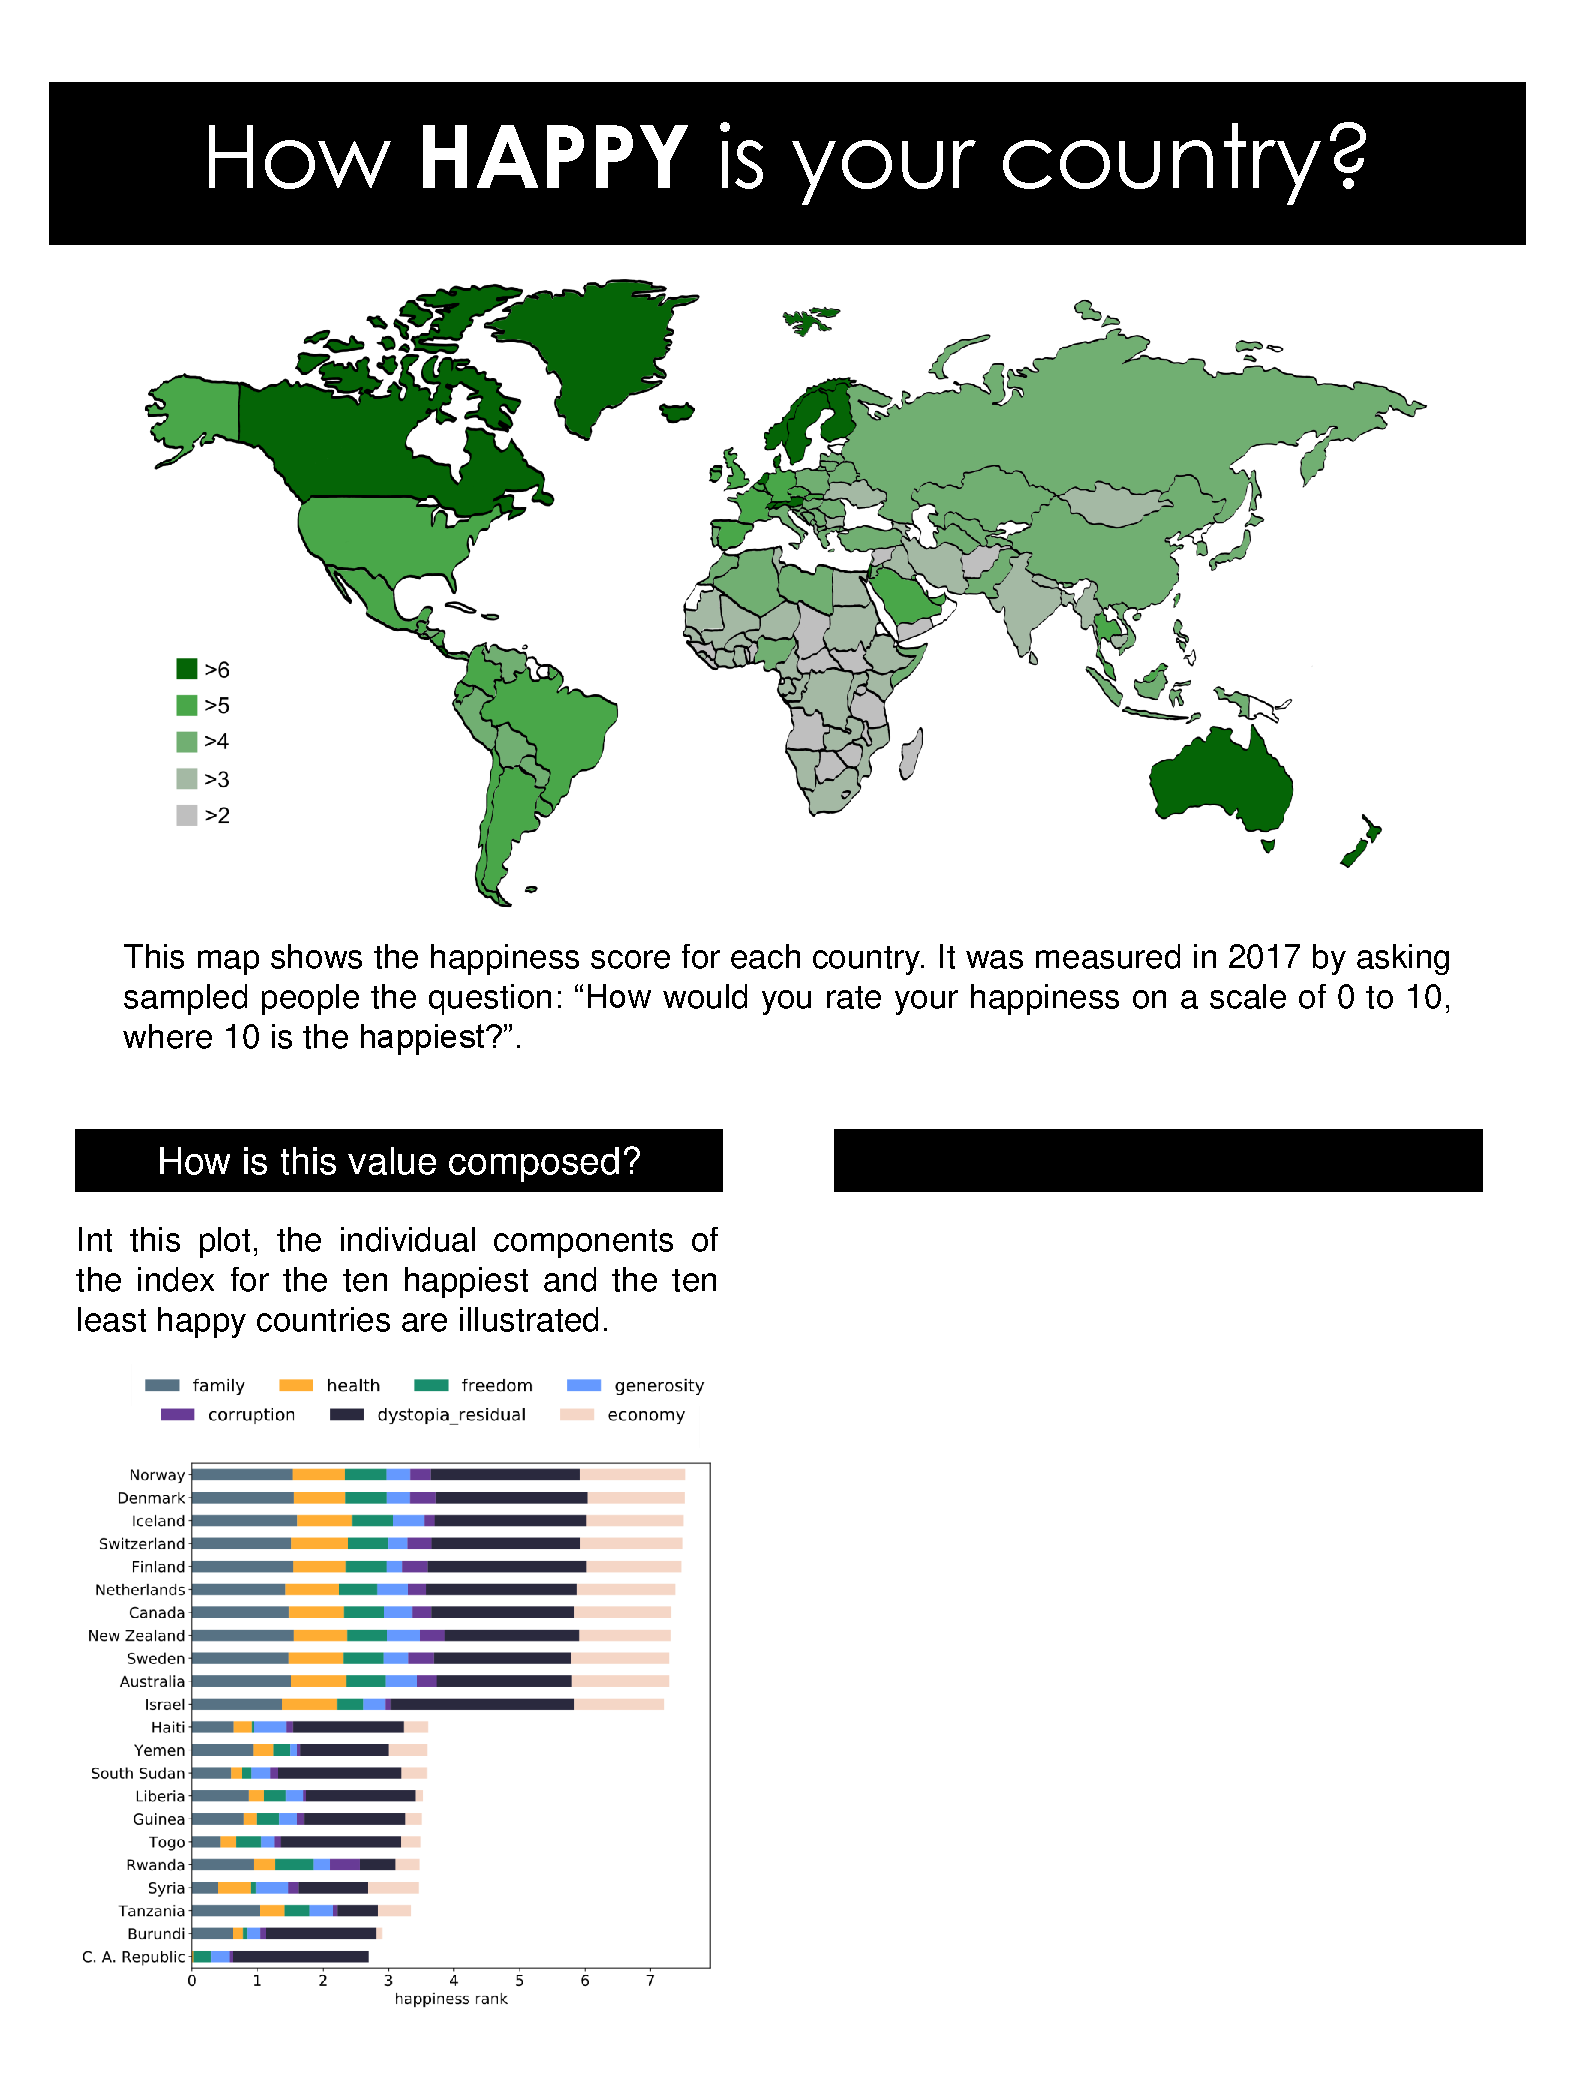
\includegraphics[width=\linewidth]{HappyPoster.pdf}}
\subsection*{(b) Evaluation}
\subsection*{(c) Bonus Points}

\end{document}
